In this chapter we present our heuristic algorithm to solve the 3D-BPPVS. 
Since the 3D-BPP is NP-Hard, an exhaustive search for a solution is not practical, therefore a heuristic search is conducted by combining the beam search algorithm described in \cref{sec:beamsearch} with the constructive heuristic described in \cref{sec:support_planes}.
In section \ref{sec:problem_state} we define the preliminary concepts that will be used in the algorithm: states, insertions and solution's feasibility.

\section{States}
\label{sec:problem_state}%
States are partial solutions of the 3D-BPPVS. Since our heuristic is based on a constructive method, starting from a state representing an empty solution we'll iteratively build new states that are always closer to a complete solution of the problem.
Being a partial solution, a state $s$ can be represented as the set of all variables present in the MILP model (\ref{sec:milp}), where some values have been fixed. We move closer to a complete solution of the problem by packing more items and opening new bins, i.e., fixing more variables.

In order to simplify the algorithm's description, we introduce a few new definitions.

\begin{definition}[Open bin]
    A bin $b \in B$ is open in state $s$ \textbf{iff}
    \begin{equation*}
        v^{s}_{b} = 1
    \end{equation*}
\end{definition}

\begin{definition}[Set of open bins]
    Let $s$ be a state, we define $B^s$ as the set of bins that are open in $s$.
    \begin{equation*}
        B^s = \{ b \in B \mid v^{s}_{b} = 1 \}
    \end{equation*}
\end{definition}

\begin{definition}[Unpacked item]
    An item $i \in I$ is unpacked in state $s$ \textbf{iff}
    \begin{equation*}
        \sum_{b \in B} u^{s}_{ib} = 0
    \end{equation*}
    ,i.e., it has yet to be assigned to an open bin.
\end{definition}

\begin{definition}[Set of unpacked items]
    Let $s$ be a state, we define $U^s$ as the set of unpacked items in $s$.
    \begin{equation*}
        U^s = \{ i \in I \mid \sum_{b \in B} u^{s}_{ib} = 0 \}
    \end{equation*}
\end{definition}

\begin{definition}[Set of packed items]
    Let $s$ be a state and let $b \in B^s$, we define $J^s_b$ as the set of items that are packed inside $b$.
    \begin{equation*}
        J^s_b = \{ i \in I \mid u^{s}_{ib} = 1 \}
    \end{equation*}
\end{definition}

Thanks to these new definitions, we can define a function that determines if a state is a final state.
\begin{definition}
    \label{def:state_final}
    A state $s$ is final if there are no more items to pack.
    \begin{equation}
        \label{algo:state_final}%
        IsFinal(s) = \left\{\begin{aligned}
            1,\hspace{0.5cm}& U^s = \emptyset \\
            0,\hspace{0.5cm}& \text{otherwise}
        \end{aligned}
        \right.
    \end{equation}
\end{definition}

We can also define the empty state, which will be used as a starting point for our algorithm.
\begin{definition}[Empty state] \label{def:empty_state}
    A state $s$ is empty if it contains a single open bin without any item packed inside.
    \begin{equation*}
        U^s = I \wedge |B^s| = 1
    \end{equation*}
    By problem definition, the first expression implies that $J^s_b = \varnothing$ $\forall b \in B^s$.
\end{definition}

Given a state $s$, for each item $i \in I$ packed in $b \in B^s$ ($i \in J^s_b$), we let $(x^s_i, y^s_i, z^s_i)$ be the coordinates of its bottom front left corner. In order to simplify the algorithm representation, rotations are handled implicitly by swapping the dimensions $w_i$ and $d_i$ of item $i \in I$ when needed. An item can have different rotations if packed in different states, therefore we use its horizontal dimensions as variables and refer to them with $w^s_i$ and $d^s_i$.

The proposed heuristic also stores additional data for each state, which will be used in the constructive heuristic described in \cref{sec:support_planes}. This additional information includes:
\begin{itemize}
    \item $Z^s_b$: the set of planes inside $b$ in state $s$. This will be described in detail in section \ref{sec:support_planes}.
    \item $T^s_b$: the AABB Tree of items packed inside $b$ in $s$. This will be described in detail in section \ref{sec:problem_state:aabbtree}.
\end{itemize}
Given a well formed state $s$ and a bin $b \in B^s$, both $J^s_b$ and $T^s_b$ contain the items packed in $b$, however adding and accessing items in $J^s_b$ has a time complexity of $O(1)$ (supposing an implementation as a hash set) while maintaining $T^s_b$ usually has a time complexity of $O(log(|J^s_b|))$. The cost of maintaining $T^s_b$ is repaid by the gain in performing checks on overlapping items, as described in the next section.

\subsection{AABB Tree}
\label{sec:problem_state:aabbtree}%

To determine the feasibility of a given state, one needs to check if no placed items overlap.
Since every item is a cuboid and our problem formulation only allows for $90\deg$ rotations over the z-axis, each item is contained inside a bounding box, which is axis-aligned.
An adequate structure to compute overlaps is then an Axis-Aligned Bounding Box Tree (AABB Tree) \citep{bergen1997efficient}.

AABB Trees are bounding volume hierarchies typically used for fast collision detection, and they usually offer a few operations:
\begin{itemize}
    \item $AABBInsert(i)$: which allows inserting an axis-aligned box $i$ in the tree,
    \item $AABBOverlaps(i)$: which allows determining if an axis-aligned box $i$ overlaps an element in the tree,
    \item $AABBClosest(i, d)$: which, given an axis-aligned box $i$ and an axis-aligned direction $d$, returns the closest element following that direction starting from the box $i$.
\end{itemize}

If the tree is appropriately balanced, each operation has a worst-case time complexity of $O(log(n))$, where $n$ is the number of elements in the tree.
Given a state $s$, maintaining an AABB Tree $T^s_b$ for each bin $b \in B^s$ allows us to do fast checks for feasibility during the construction of a solution (as detailed in \ref{ssec:scoring_insertions}) and fast feasibility checks on the final states for error detection.

\label{aabb:get_supporting}%
An additional opertation $AABBGetSupporting(i, \beta_s)$ was added to compute the set of supporting boxes of item $i$ given a vertical tolerance $\beta_s$.
This was possible by checking intersections over the XY-plane, similarly to the $AABBOverlaps$ implementation, and keeping items that are below $i$ with a distance within tolerance.

\subsection{Insertions}
\label{sec:problem_state:insertions}%

Our algorithm is based on the constructive heuristic described in section \ref{sec:support_planes}. Starting from an empty bin, it places items inside the open bins until no more items are available. We model the concept of placing a set of unpacked items inside an open bin as an insertion.
\begin{definition}[Insertion]
    \label{def:insertion}%
    Let $s$ be a state, we define an insertion $p$ as a tuple $(b_p, I_p)$ where $b_p \in B^s$, and $I_p \subseteq U^s$. Such a tuple represents the placement of items from $I_p$ in bin $b_p$ at coordinates $(x^s_i, y^s_i, z^s_i)$ $\forall i \in I_p$.
\end{definition}
\begin{observation}
    \label{oss:state_bin_open}
    Given a state $s$ and an insertion $p = (b, \emptyset)$ where $b \notin B^s$, $p$ is an insertion that opens a new bin $b$ in $s$.
\end{observation}
\begin{observation}[Same z insertion]
    \label{obs:same_z_insertion}
    In our algorithm we will always insert items on the same "plane", that is with the same z coordinate. Let $p = (b_p, I_p)$ be an insertion, then:
    \begin{equation}
        \exists z (z \in \{0,..,H\} \land \forall i ( i \in I_p \implies z^s_i = z))
    \end{equation}
\end{observation}
To perform an insertion $p = (b_p, I_p)$ means placing all the items from $I_p$ inside the bin $b_p$. Performing $p$ on a state $s$ generates a new state $s'$. This, however, is an expensive operation: it requires cloning the state, a heavy time-consuming and memory-intensive task, and updating all the related data structures with a time complexity of $O(|I_p|log(|J^s_{b_p}|))$ (dominated by the update of the AABB Tree $T^s_{b_p}$). 

In our algorithm, starting from a feasible state $s$, we generate multiple new states $s'$ by performing different insertions on $s$. These new states are then evaluated (as described in section \ref{ssec:scoring_states}) and only some of the best ones are retained for the rest of the process. To avoid performing insertions on states that will be discarded, we divide the insertion process in two phases: the first phase enables us to compute the score of a state without updating all its data structures, while the second phase actually performs the updates but only on the retained states. 

Let us define the concept of pending insertion.
\begin{definition}[Pending insertion]
    We define $p^s$ as the insertion that is pending on state $s$. A pending insertion is an insertion that in the future will be applied to its state.
\end{definition}
The first phase of the insertion process consists in the application of the $Next$ operator.
\begin{definition}[Next]
    \label{def:state_next}%
    Let $p$ be an insertion over a state $s$, we define $s^\prime = Next(s, p)$ as a shallow copy of $s$ where $p$ is the pending insertion ($p^{s'} = p$).
\end{definition}
Creating a shallow copy of a state means creating a copy of such a state without cloning it in memory. For each new state $s'$ obtained in this way, we compute its score by considering the effects of a future application of $p_{s'}$. After evaluating all states and selecting the best ones, we proceed with the second phase of the insertion process, which is the $Commit$ of pending insertions. This operation copies the states in memory and updates all the relevant data structures. The $Commit$ scheme is shown in Algorithm \ref{algo:state_commit}.

\begin{algorithm}[H] \label{algo:state_commit}
    \DontPrintSemicolon
    \SetAlgoLined
    \SetKwInOut{Input}{input}
    \SetKwInOut{Output}{output}
    \Input{$s$}
    \Output{$s^\prime$}
    $(b, I) \gets s.p$\;
    $s^\prime \gets Clone(s)$\CommentSty{ //Memory clone of $s$}\;
    \If{$b \in s^\prime.B$}{
        $q_b \gets (q_i \in s^\prime.Q : i = b)$\;
        $q_b.J \gets q_b.J \cup I$\;
        $s^\prime.U \gets s^\prime.U \setminus I$\;
    }
    \Else(Open a new bin){
        $s^\prime.B \gets s^\prime.B \cup b$\;
        $s^\prime.Q \gets s^\prime.Q \cup OpenBin(b)$\;
    }
    $s^\prime.p \gets \text{none}$\;
    \Return{$s^\prime$}
    \caption{Commit}
\end{algorithm}

\subsection{Feasibility}
\label{sec:problem_state:feasibility}%
A state $s$ is feasible if, for each bin $b \in B^s$:
\begin{itemize}
    \item items in $J^s_b$ do not overlap among themselves,
    \item all items in $J^s_b$ are placed within the bin's bounds,
    \item each item in $J^s_b$ is either on the ground or satisfies at least one of the support conditions (cond. \ref{support:area_support}, cond. \ref{support:vertex_support}).
\end{itemize}
Since the proposed heuristic is constructive, we start with an initial feasible state and generate new states by applying insertions that maintain feasibility. It is therefore more convenient to define the concept of feasibility relatively to an insertion.

\paragraph*{Insertion feasibility}
An insertion $p = (b_p, I_p)$ that is pending on a given state $s$ is feasible if every inserted item $i \in I_p$ satisfies the constraint of non-overlap (\ref{cons:no_overlap}, both with items placed in $J^s_{b_p}$ and with other items in $I_p$), the constraint of support (\ref{cons:every_item_is_supported}) and if it is placed within the bin.
Let $I_{\text{support}}$ be the set of items that could support item $i$, computed through the AABB tree $T^s_{b_p}$ as defined in \cref{aabb:get_supporting}.
Let $HasSupport(i, I_{\text{support}})$ be a function that returns true if the considered item would verify at least one of the support conditions (cond. \ref{support:area_support} or cond. \ref{support:vertex_support}) and false otherwise.
We define a function $IsFeasible(i, I_{\text{support}}, T^s_{b_p})$ which returns true if the insertion of $i$ in bin $b_p$ for state $s$ is feasible, and false otherwise.
If every item $i \in I_p$ is feasible then insertion $p$ is feasible.
In case the insertions of some items in $I_p$ aren't feasible, we can always define a function $RemoveInfeasibleItems(p, I_{\text{support}}, T^s_{b_p})$ which removes every unfeasible item from $I_p$ and returns a new insertion $p^\prime = (b_p, I_{p^\prime})$ where:
\begin{equation*}
    I_{p^\prime} = I_p \setminus \{i \in I_p : \lnot IsFeasible(i, I_{\text{support}}, T^s_{b_p})\}. \label{algo:remove_infeasible}
\end{equation*}

Checking if a state is feasible can then be done by iteratively applying all the insertions ordered by z and updating the proper data structures.
\begin{proposition}
    \label{prop:feasible_expansion}
    A state $s^\prime$ derived by committing a feasible insertion $p$ to a feasible state $s$ is always feasible.
\end{proposition}
This proposition is true by construction of insertions $p$, and combined with observation \ref{def:empty_state_feasible} it proves that our constructive heuristic always maintains feasible solutions. 
\begin{observation}
    \label{def:empty_state_feasible}
    Let $s_e$ be an empty state as stated in definition \ref{def:empty_state}, then it is feasible.
\end{observation}

\subsection{State Hashing}
\label{sec:state_uniqueness}%
From a given state, it is possible to apply two different sequences of insertions and end up with two states that have the same items in the same positions.
This undesirable behavior was observed during our computational experiments.
We develop a hashing mechanism that enables checking if two states are likely the same in constant time.
In a state $s$, we can uniquely identify a packed item $i \in J^s_b$ in a given position $(x^s_i, y^s_i, z^s_i)$ with its given dimensions $(w^s_i, d^s_i, h_i)$ with a non-commutative hashing function $hash\_nc$. The resulting hash $hash_{ib} = hash\_nc(b, x^s_i, y^s_i, z^s_i, w^s_i, d^s_i, h_i)$ can identify every equivalent packing of an item of the same shape in that specific bin spot.
Since $hash_{ib}$ identifies one item with the shape of $i$ in the same spot as $i$, we can use a commutative function to combine every hash for every packed item in every bin to ignore the order with which items were added to the solution.
The combined hash can then be saved inside our state structures as follows.
\begin{equation}
    hash^s = \sum\limits_{b \in B^s}{\sum\limits_{i \in J^s_b}{hash_{ib}}}
\end{equation}
In our tests, by filtering states with the proposed hash as seen in Algorithm \ref{algo:beamsearch} with a simple 64-bit hashing function, we were able to filter out all equal states between iterations with a low amount of collisions.
Since the combination of hashes is a simple sum with modulus, the hashing of a state can also be kept updated in constant time at each iteration by simply adding the inserted hashes in the $Commit$ function (Algorithm \ref{algo:state_commit}).

\section{Beam Search}
\label{sec:beamsearch}%
Beam Search (BS) is a heuristic tree search algorithm designed for systems with limited memory, where expanding every possible node is unfeasible.
The idea behind BS is to conduct an iterative truncated breadth-first search where, at each iteration, only a limited number $k$ of nodes is expanded.
After the expansion, every new node is evaluated and the $k$ best nodes are retained for the next iteration. The algorithm keeps exploring the solution tree until no further node can be expanded.

To perform BS one must define the node structure, an expansion function to generate new nodes from existing ones, a ranking between nodes, and a function to determine if a node is final.

A node in the tree can be represented as a state, as described in  \cref{sec:problem_state}, and \cref{algo:state_final} can be used to determine if a state is final. We also know that a new state $s^\prime$ derived by $s$ by applying a feasible insertion $p$ can be computed as in \cref{sec:problem_state:insertions}.
This state expansion procedure, with the exception of empty insertions, will generate new states in our tree which will add a positive number of bins or packed items to the solution. This procedure, eventually, will converge and generate a final state.

If the starting state for the search is feasible, every new generated state will be feasible and if a final state is found it will be feasible (\cref{prop:feasible_expansion}).
States are expanded by generating insertions and applying such insertions to them, following the two phase procedure outlined in \cref{sec:problem_state:insertions}. In our BS, the first phase is performed before the evaluation of each new state while the second phase is performed only after the selection of the $k$ best states.
As noted in \cref{sec:state_uniqueness}, since by evaluating different insertions on different states it is possible to end up having two equal states, a filtering mechanism based on hashing is introduced.
During each iteration, it is possible to keep the hashes of the best selected states in a hash set and discard new states with the same hash.

Given a set of initial states $S^0$ and the number of best states to expand at each iteration $k$, the described BS is described in Algorithm \ref{algo:beamsearch}.
As observed in \cref{def:empty_state}, it's possible to start the search from $S^0 = \{ s_e \}$.

\begin{algorithm}[H] \label{algo:beamsearch}
    \DontPrintSemicolon
    \SetAlgoLined
    \SetKwInOut{Input}{input}
    \SetKwInOut{Output}{output}
    \Input{$S^0, k$}
    \Output{$s_{best}$}
    $S^t \gets S^0$\;
    $S_{final} \gets \emptyset$\;
    \Repeat{$S^t \neq \emptyset $}{
        $S^{t+1} \gets Expand(S^t)$ (algo. \ref{algo:state_successor})\;
        $S_{final} \gets S_{final} \cup \{s \in S^{t+1} : IsFinal(s)\}$ (def. \ref{def:state_final})\;
        $S^{t+1} \gets S^{t+1} \setminus S_{final}$\;
        $S^{t+1} \gets Sort(S^{t+1})$ (sec. \ref{ssec:scoring_states})\;
        $S^t \gets \emptyset$\;
        $i \gets 0$\;
        $seen \gets \emptyset$\;
        \ForAll{$s \in S^{t+1}$}{
            \If{$hash^s \in seen$}{
                continue\;
            }
            $S^t \gets S^t \cup Commit(s)$ (algo. \ref{algo:state_commit})\;
            $seen \gets seen \cup \{ hash^s \}$\;
            $i \gets i+1$\;
            \If{$i > k$}{
                break\;
            }
        }
    }
    $S_{final} \gets Sort(S_{final})$\;
    \Return{best element of $S_{final}$}
    \caption{Beam search}
\end{algorithm}

\paragraph*{State Expansion}

An expansion of a state $s$ is a new set of states $S_{new}$ obtained by applying a set of feasible insertions to $s$. In order to determine these insertions, an underlying heuristic is used (described in \cref{sec:support_planes}).

The main idea in this phase of the algorithm is to find feasible insertions in all the bins in $B^s$ at the lowest possible height, for each item in $U^s$. 
To reduce the number of possible expansions to evaluate, we limit the search only to insertions of items with unique shapes.
With a similar concept to the one used in \cref{sec:state_uniqueness}, we compute an hash for each item's dimensions and then use it to group items that have the same shape.
The evaluation of new insertions can then be done with two different approaches:
\begin{itemize}
    \label{def:placement_modes}%
    \item \textbf{PS}: (single placement) where we evaluate only the insertion of a single item per item type. This generates insertions of at most 1 item.
    \item \textbf{PM}: (multiple placement) where we evaluate the biggest possible insertion of a group of items of the same shape. This generate insertions of at most the size of the considered group of items with the same shape.
\end{itemize}
Creating insertions of groups of similar items is a common strategy in Pallet Loading Problems (e.g., \cite{elhedhli2019three}) to create better bases of support for upper layers.
With a similar intuition, the idea of placing groups of items of the same shape is to facilitate the creation of uniform planes to be used to support future insertions.

Given a set of items $I$ and a tolerance $\beta_s$, we can introduce an algorithm to group the items by their shape and produce a set $G$ of tuples $(h, I^\prime)$, where $h$ is the hash summarizing the shape of the group and $I^\prime$ is the set of items grouped. This procedure is described in Algo. \ref{algo:group_by_hash}.
Once items are grouped by shape, the best insertion for each class of items is computed for each open bin. If no insertion is possible in any bin, then the only viable insertion is the bin opening insertion (\cref{oss:state_bin_open}).
The state expansion procedure is detailed in Algo. \ref{algo:state_successor}. The algorithm is described in PM mode, however minor modifications are needed to switch to PS mode.

\begin{algorithm}[H] \label{algo:state_successor}
    \DontPrintSemicolon
    \SetAlgoLined
    \SetKwInOut{Input}{input}
    \SetKwInOut{Output}{output}
    \Input{$S$}
    \Output{$S_{new}$}
    \ForAll{$s \in S$}{
        $S_{new} \leftarrow \emptyset$\;
        $I_{family} \leftarrow GroupByFamily(s.Unpacked)$\;
        %$minPlacement \leftarrow \{(b, 0) | \forall b \in s.Bins \}$\;
        $placed \leftarrow false$\;
        \ForAll{$(family, I) \in I_{family}$}{
            \ForAll{$bin \in s.Bins$}{
                $placement \leftarrow SPBestInsertion(s, bin, I)$ (Algorithm \ref{algo:sp_bestinsertion})\;
                \If{$placement \neq \emptyset$}{
                    $placed \leftarrow true$\;
                    %$minPlacement(bin) \leftarrow min(minPlacement(bin), placement.z)$\;
                    %TODO: abuso di notazione
                    $S_{new} \leftarrow S_{new} \cup Next(s, placement)$\;
                }
            }
        }
        \If{$placed = false$}{
            $S_{new} \leftarrow S_{new} \cup OpenNewBin(s)$\;
        }
        %TODO: Filter?
    }
    \Return{$S_{new}$}
    \caption{Expand}
\end{algorithm}
\begin{algorithm}[ht] \label{algo:group_by_hash}
    \DontPrintSemicolon
    \SetAlgoLined
    \SetKwInOut{Input}{input}
    \SetKwInOut{Output}{output}
    \Input{$I$}
    \Output{$G$}
    $G \gets \emptyset$\;
    \ForAll{$i \in I$}{
        $generate \gets \text{true}$\;
        \ForAll{$(h, I^\prime) \in G$}{
            \If{$h = hash(w_i, d_i, h_i)$}{
                $generate \gets \text{false}$\;
                $I^\prime \gets I^\prime \cup i$\;
                break\;
            }
        }
        \If{$generate = \text{true}$}{
            $G \gets G \cup (hash(w_i, d_i, h_i), \{ i \})$\;
        }
    }
    \Return{$G$}
    \caption{Group By Hash}
\end{algorithm}


\subsection{Sorting States}
\label{ssec:scoring_states}%
In order to sort states, an ordering needs to be defined over them.
Since the selection of a state over another is what will influence the final solution the most, parameters that are directly related to minimizing the objective function are used.

In the proposed solution, we use lexicographic ordering to handle multiple objective functions.
\begin{definition}
    \label{def:lexicographic_ordering}
    Let $f_1(s), f_2(s), f_i(s), \dots, f_n(s)$ be objective functions ordered by precedence based on index $i \in \mathbb{Z}$, then 
    \begin{equation*}
        s < s^\prime \hspace{.2cm} \textbf{iff} \hspace{.2cm} \exists j \in \mathbb{Z} : \left\{
            \begin{aligned}
                f_j(s) < f_j(s^\prime) & \\
                f_k(s) = f_k(s^\prime) &,\hspace{.5cm} \forall k \in \mathbb{Z} : 0 \le k < j 
            \end{aligned}
        \right.
    \end{equation*}
\end{definition}

Scoring metrics for each state $s$ that we want to evaluate can then be computed in the $Next$ algorithm by considering the contents of the pending insertions and updating each objective function value differentially.

We use the following objective functions (considering a minimization direction):
\begin{itemize}
    \item $f_1(s) = |B^s|$: we prefer states that opened fewer bins.
    \item $f_2(s) = -\text{avgvol}(s)$: we prefer states that have packed more average volume between bins.
    \item $f_3(s) = -\text{avgcageratio}(s)$: we prefer states that have better average cage ratio (\cref{eq:cage_ratio}) between bins.
\end{itemize}

\section{Support Planes}
\label{sec:support_planes}%
Support Planes (SP) is a constructive heuristic for the 3D-BPPVS which is based on an underlying 2D-BPP heuristic. The latter is used to generate feasible insertions inside a bin starting from a set of items to pack.
Since insertions must be feasible, SP maintains an internal data structure to facilitate feasibility checks.
The idea at the base of SP is to build a solution to the 3D-BPP by filling 2D planes called \textit{support planes}.

Each support plane is a tuple $(z, I_{support}, I_{upper})$ where
\begin{itemize}
    \item $z$: is the height of the plane,
    \item $I_{support}$: the set of the items that can offer support to items placed on the plane,
    \item $I_{upper}$: the set of items that will be obstacles to potential new items placed on the plane.
\end{itemize}

Every item placed in the bin can either generate a new support plane or be part of the supporting items of other planes.
Items placed above a particular plane, such that $z_i + h_i > z$, are considered obstacles and are added to the $I_{upper}$ set.
When creating new insertion, given a set of items to place $I$, SP selects the first feasible insertion starting from the lowest plane by using a modified version of the Extreme Point algorithm (\cite{crainic2008extreme}) that works in two dimensions.
Once no more insertions can be made on the lowest available support plane, it is removed from the set of planes.
Since insertions always happen in the lowest possible planes, the set of obstacles of those planes is composed of items that have only their top face above the $z$ of the evaluated plane, such that $z_i \le z < z_i + h_i$.

The standard Extreme Point (EP) heuristic evaluates the placement of rectangles in a plane based on a set of reference points with a best-fit approach.
Each rectangle placement generates a new set of reference points which are usually introduced based on the projection of its corner points along the orthogonal axis of the plane.
The corner points of an added rectangle $r$ placed in $(x_r, y_r)$ of dimensions $(w_r, d_r)$ are the top left corner $(x_r, y_r + d_r)$ and the bottom right corner $(x_r + w_r, y_r)$.
In our version of the algorithm, however, the corner points of each item are introduced without projecting them to increase the likelihood of generating placements that verify the support constraint.
Placements follow a first-fit approach where the algorithm selects the first point closest to the origin where a rectangle can fit with or without rotations.
In order to facilitate the evaluation of reference points with support, we also generate a reference point in the bottom left corner of each item that belongs to the set of supporting items $I_{support}$.
When a reference point is used for a placement, it is then removed from the pool of reference points.
Before evaluating placements, the item to place are ordered based on their area (this is meaningful only in multiple placements PM mode).
New planes have always the origin of space $(0,0)$ as a first reference point.

Since reference points are usually ordered based on the euclidean distance from the bottom left corner of the plane and the corner points are usually generated and projected towards the origin of each axis, the placements over one plane are usually biased towards the bottom left corner.
To address the problem, whenever we are generating 2D placements, we evaluate four instances of EP where each one has a different coordinate change that moves the plane's origin to a different corner of the bin.
This addition is based on similar approaches from the literature where it is used to distribute weight more uniformly across a surface (ex. \cite{GAJDA2022102559}), and it was proved to yield better cage ratio results in our computational experiments.

The EP procedure is called for each item to pack on a given plane.
In order to produce a valid insertion $p$, every item in $I_p$ should not overlap with other items in $I_p$ (as stated in \cref{def:insertion}).
Since the AABB tree for a given state is shared by each evaluation of a possible insertion, it cannot be modified to account for temporary placements of items.
This means that we need to keep a temporary AABB tree updated composed of the items that are part of the current insertion $T^\prime_p$.
We can then define a function that uses the temporary tree and the feasibility function defined in \cref{sec:problem_state:feasibility} to ensure that we are producing a feasible insertion as \cref{eq:ep_can_pack}.
\begin{equation}
    \label{eq:ep_can_pack}
    EPCanPack(i, I_{support}, T^s_{b_p}, T^\prime_p) = IsFeasible(i, I_{support}, T^s_{b_p}) \land \lnot AABBOverlaps(i, T^\prime_p)
\end{equation}
A graphical representation of a support plane is shown in \cref{fig:support_planes}, with the reference points available. In \cref{fig:ep_coordinate_changes} the state of two extreme point instances for the bottom left and top left coordinate changes are shown.
When a bin is opened, the only support plane available is the one on the ground.
In the figure different coordinate changes are marked with different colors.

\begin{figure}[hp]
    \centering
    \scalebox{0.9}{%
    

\tikzset{every picture/.style={line width=0.75pt}} %set default line width to 0.75pt        

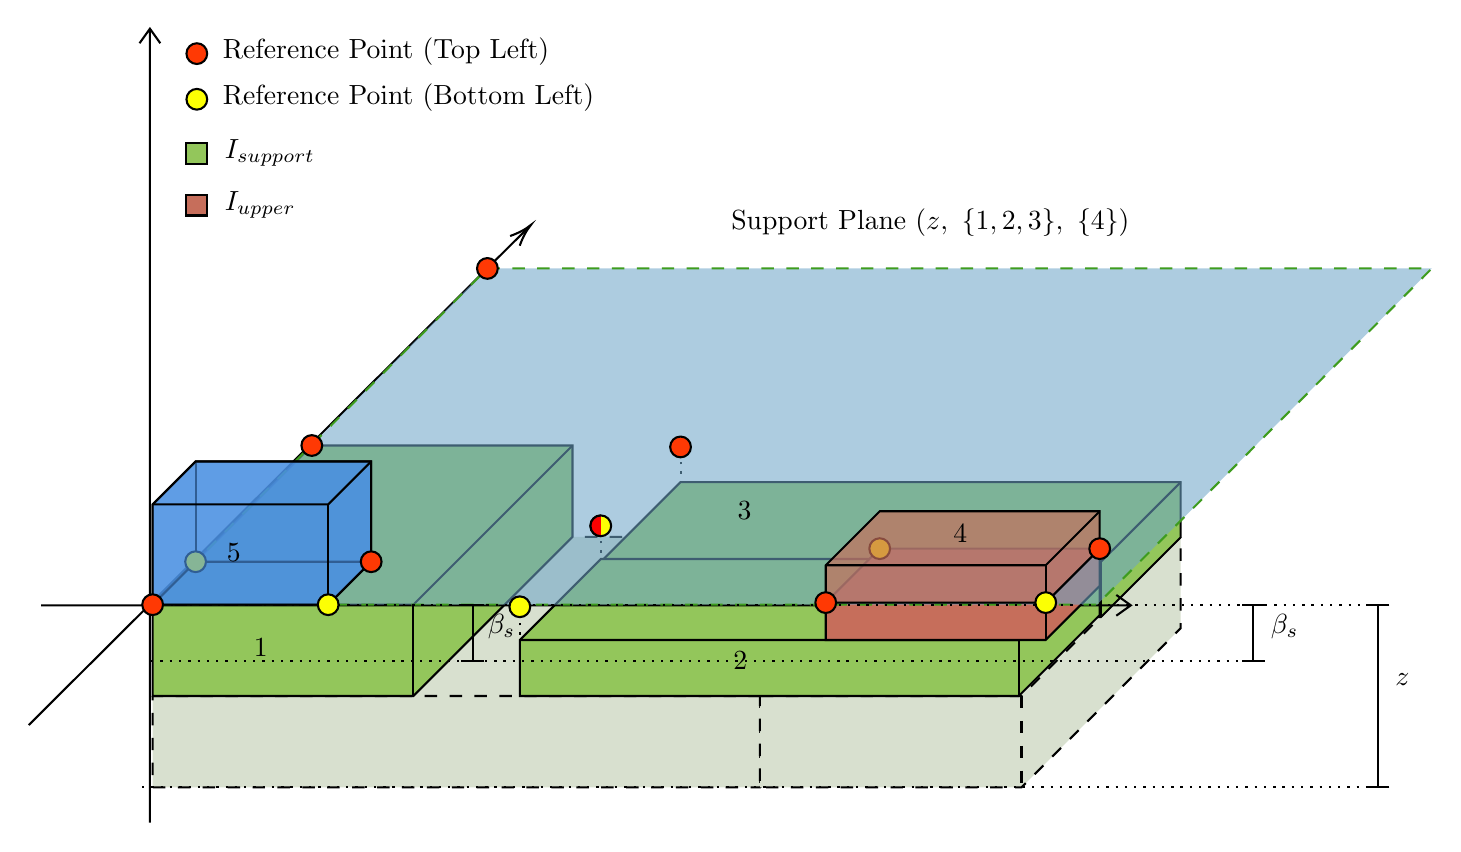
\begin{tikzpicture}[x=0.75pt,y=0.75pt,yscale=-1,xscale=1]
%uncomment if require: \path (0,412); %set diagram left start at 0, and has height of 412

%Shape: Cube [id:dp7106500856615827] 
\draw  [fill={rgb, 255:red, 216; green, 224; blue, 207 }  ,fill opacity=1 ][dash pattern={on 4.5pt off 4.5pt}] (69.7,334.5) -- (146.4,257.81) -- (439,257.81) -- (439,301.81) -- (362.31,378.5) -- (69.7,378.5) -- cycle ; \draw  [dash pattern={on 4.5pt off 4.5pt}] (439,257.81) -- (362.31,334.5) -- (69.7,334.5) ; \draw  [dash pattern={on 4.5pt off 4.5pt}] (362.31,334.5) -- (362.31,378.5) ;
%Straight Lines [id:da8316956251676535] 
\draw  [dash pattern={on 0.84pt off 2.51pt}]  (285.62,269.89) -- (285.62,252.5) ;
%Straight Lines [id:da38384433092333237] 
\draw  [dash pattern={on 0.84pt off 2.51pt}]  (324.05,231.89) -- (324.05,214.5) ;
%Shape: Cube [id:dp47709739603214574] 
\draw  [fill={rgb, 255:red, 216; green, 224; blue, 207 }  ,fill opacity=1 ][dash pattern={on 4.5pt off 4.5pt}] (362.31,334.5) -- (439,257.81) -- (565,257.81) -- (565,301.81) -- (488.31,378.5) -- (362.31,378.5) -- cycle ; \draw  [dash pattern={on 4.5pt off 4.5pt}] (565,257.81) -- (488.31,334.5) -- (362.31,334.5) ; \draw  [dash pattern={on 4.5pt off 4.5pt}] (488.31,334.5) -- (488.31,378.5) ;
%Shape: Cube [id:dp7977002200403227] 
\draw  [fill={rgb, 255:red, 147; green, 198; blue, 91 }  ,fill opacity=1 ] (69.7,290.5) -- (146.4,213.81) -- (272,213.81) -- (272,257.81) -- (195.31,334.5) -- (69.7,334.5) -- cycle ; \draw   (272,213.81) -- (195.31,290.5) -- (69.7,290.5) ; \draw   (195.31,290.5) -- (195.31,334.5) ;
%Shape: Cube [id:dp7121611670665484] 
\draw  [fill={rgb, 255:red, 147; green, 198; blue, 91 }  ,fill opacity=1 ] (285.62,269.89) -- (324.05,231.46) -- (565,231.46) -- (565,258.06) -- (526.56,296.5) -- (285.62,296.5) -- cycle ; \draw   (565,231.46) -- (526.56,269.89) -- (285.62,269.89) ; \draw   (526.56,269.89) -- (526.56,296.5) ;
%Shape: Cube [id:dp604763542929154] 
\draw  [fill={rgb, 255:red, 147; green, 198; blue, 91 }  ,fill opacity=1 ] (246.62,307.5) -- (285.62,268.5) -- (526,268.5) -- (526,295.5) -- (487,334.5) -- (246.62,334.5) -- cycle ; \draw   (526,268.5) -- (487,307.5) -- (246.62,307.5) ; \draw   (487,307.5) -- (487,334.5) ;
%Shape: Axis 2D [id:dp786981943451631] 
\draw  (16,290.81) -- (541,290.81)(68.4,13) -- (68.4,395.5) (534,285.81) -- (541,290.81) -- (534,295.81) (63.4,20) -- (68.4,13) -- (73.4,20)  ;
%Straight Lines [id:da31524103851047525] 
\draw    (10,348.5) -- (250.58,108.91) ;
\draw [shift={(252,107.5)}, rotate = 135.12] [color={rgb, 255:red, 0; green, 0; blue, 0 }  ][line width=0.75]    (10.93,-3.29) .. controls (6.95,-1.4) and (3.31,-0.3) .. (0,0) .. controls (3.31,0.3) and (6.95,1.4) .. (10.93,3.29)   ;
%Shape: Cube [id:dp6424617162036526] 
\draw  [fill={rgb, 255:red, 198; green, 110; blue, 91 }  ,fill opacity=1 ] (394,289.5) -- (420,263.5) -- (526,263.5) -- (526,281.5) -- (500,307.5) -- (394,307.5) -- cycle ; \draw   (526,263.5) -- (500,289.5) -- (394,289.5) ; \draw   (500,289.5) -- (500,307.5) ;
%Shape: Parallelogram [id:dp3639839698249763] 
\draw  [color={rgb, 255:red, 62; green, 156; blue, 30 }  ,draw opacity=1 ][fill={rgb, 255:red, 110; green, 165; blue, 200 }  ,fill opacity=0.57 ][dash pattern={on 4.5pt off 4.5pt}] (231,128.5) -- (686,128.5) -- (524.7,290.5) -- (69.7,290.5) -- cycle ;
%Straight Lines [id:da11997650250706615] 
\draw    (659.96,290.5) -- (659.96,378.5) ;
\draw [shift={(659.96,378.5)}, rotate = 270] [color={rgb, 255:red, 0; green, 0; blue, 0 }  ][line width=0.75]    (0,5.59) -- (0,-5.59)   ;
\draw [shift={(659.96,290.5)}, rotate = 270] [color={rgb, 255:red, 0; green, 0; blue, 0 }  ][line width=0.75]    (0,5.59) -- (0,-5.59)   ;
%Straight Lines [id:da7479086158615895] 
\draw  [dash pattern={on 0.84pt off 2.51pt}]  (69.7,290.5) -- (665,290.5) ;
%Straight Lines [id:da00936893511639092] 
\draw  [dash pattern={on 0.84pt off 2.51pt}]  (64.66,378.5) -- (659.96,378.5) ;
%Straight Lines [id:da2603505755036556] 
\draw  [dash pattern={on 0.84pt off 2.51pt}]  (69,317.5) -- (600,317.5) ;
%Straight Lines [id:da21695403696781168] 
\draw    (600,290.5) -- (600,317.5) ;
\draw [shift={(600,317.5)}, rotate = 270] [color={rgb, 255:red, 0; green, 0; blue, 0 }  ][line width=0.75]    (0,5.59) -- (0,-5.59)   ;
\draw [shift={(600,290.5)}, rotate = 270] [color={rgb, 255:red, 0; green, 0; blue, 0 }  ][line width=0.75]    (0,5.59) -- (0,-5.59)   ;
%Straight Lines [id:da17628222853988207] 
\draw    (224,290.5) -- (224,317.5) ;
\draw [shift={(224,317.5)}, rotate = 270] [color={rgb, 255:red, 0; green, 0; blue, 0 }  ][line width=0.75]    (0,5.59) -- (0,-5.59)   ;
\draw [shift={(224,290.5)}, rotate = 270] [color={rgb, 255:red, 0; green, 0; blue, 0 }  ][line width=0.75]    (0,5.59) -- (0,-5.59)   ;
%Shape: Cube [id:dp458320338188952] 
\draw  [fill={rgb, 255:red, 74; green, 144; blue, 226 }  ,fill opacity=0.66 ] (175,269.8) -- (154.3,290.5) -- (69.7,290.5) -- (69.7,242.2) -- (90.4,221.5) -- (175,221.5) -- cycle ; \draw   (69.7,290.5) -- (90.4,269.8) -- (175,269.8) ; \draw   (90.4,269.8) -- (90.4,221.5) ;
%Shape: Circle [id:dp9728798663710179] 
\draw  [fill={rgb, 255:red, 252; green, 255; blue, 4 }  ,fill opacity=1 ] (86,47) .. controls (86,44.24) and (88.24,42) .. (91,42) .. controls (93.76,42) and (96,44.24) .. (96,47) .. controls (96,49.76) and (93.76,52) .. (91,52) .. controls (88.24,52) and (86,49.76) .. (86,47) -- cycle ;
%Shape: Circle [id:dp41733873180988235] 
\draw  [fill={rgb, 255:red, 252; green, 255; blue, 4 }  ,fill opacity=1 ] (85.4,269.8) .. controls (85.4,267.04) and (87.64,264.8) .. (90.4,264.8) .. controls (93.17,264.8) and (95.4,267.04) .. (95.4,269.8) .. controls (95.4,272.56) and (93.17,274.8) .. (90.4,274.8) .. controls (87.64,274.8) and (85.4,272.56) .. (85.4,269.8) -- cycle ;
%Shape: Cube [id:dp9609158816144449] 
\draw  [fill={rgb, 255:red, 74; green, 144; blue, 226 }  ,fill opacity=0.66 ] (69.7,242.2) -- (90.4,221.5) -- (175,221.5) -- (175,269.8) -- (154.3,290.5) -- (69.7,290.5) -- cycle ; \draw   (175,221.5) -- (154.3,242.2) -- (69.7,242.2) ; \draw   (154.3,242.2) -- (154.3,290.5) ;
%Shape: Circle [id:dp7069570068237806] 
\draw  [fill={rgb, 255:red, 252; green, 255; blue, 4 }  ,fill opacity=1 ] (149.3,290.5) .. controls (149.3,287.74) and (151.54,285.5) .. (154.3,285.5) .. controls (157.06,285.5) and (159.3,287.74) .. (159.3,290.5) .. controls (159.3,293.26) and (157.06,295.5) .. (154.3,295.5) .. controls (151.54,295.5) and (149.3,293.26) .. (149.3,290.5) -- cycle ;
%Shape: Circle [id:dp07493756825553233] 
\draw  [fill={rgb, 255:red, 252; green, 255; blue, 4 }  ,fill opacity=1 ] (241.62,291.5) .. controls (241.62,288.74) and (243.86,286.5) .. (246.62,286.5) .. controls (249.38,286.5) and (251.62,288.74) .. (251.62,291.5) .. controls (251.62,294.26) and (249.38,296.5) .. (246.62,296.5) .. controls (243.86,296.5) and (241.62,294.26) .. (241.62,291.5) -- cycle ;
%Shape: Circle [id:dp9652867077591403] 
\draw  [fill={rgb, 255:red, 252; green, 255; blue, 4 }  ,fill opacity=1 ] (280.62,252.5) .. controls (280.62,249.74) and (282.86,247.5) .. (285.62,247.5) .. controls (288.38,247.5) and (290.62,249.74) .. (290.62,252.5) .. controls (290.62,255.26) and (288.38,257.5) .. (285.62,257.5) .. controls (282.86,257.5) and (280.62,255.26) .. (280.62,252.5) -- cycle ;
%Straight Lines [id:da7143423337159592] 
\draw  [dash pattern={on 0.84pt off 2.51pt}]  (246.62,313.89) -- (246.62,296.5) ;
%Shape: Rectangle [id:dp672375593139905] 
\draw  [fill={rgb, 255:red, 147; green, 198; blue, 91 }  ,fill opacity=1 ] (86,68) -- (96,68) -- (96,78) -- (86,78) -- cycle ;
%Shape: Rectangle [id:dp16133242915286994] 
\draw  [fill={rgb, 255:red, 198; green, 110; blue, 91 }  ,fill opacity=1 ] (86,93) -- (96,93) -- (96,103) -- (86,103) -- cycle ;
%Shape: Circle [id:dp7335317400317659] 
\draw  [fill={rgb, 255:red, 255; green, 57; blue, 4 }  ,fill opacity=1 ] (86,25) .. controls (86,22.24) and (88.24,20) .. (91,20) .. controls (93.76,20) and (96,22.24) .. (96,25) .. controls (96,27.76) and (93.76,30) .. (91,30) .. controls (88.24,30) and (86,27.76) .. (86,25) -- cycle ;
%Shape: Circle [id:dp4790782266696906] 
\draw  [fill={rgb, 255:red, 255; green, 57; blue, 4 }  ,fill opacity=1 ] (319.05,214.5) .. controls (319.05,211.74) and (321.29,209.5) .. (324.05,209.5) .. controls (326.82,209.5) and (329.05,211.74) .. (329.05,214.5) .. controls (329.05,217.26) and (326.82,219.5) .. (324.05,219.5) .. controls (321.29,219.5) and (319.05,217.26) .. (319.05,214.5) -- cycle ;
%Shape: Circle [id:dp3675058769915285] 
\draw  [fill={rgb, 255:red, 255; green, 57; blue, 4 }  ,fill opacity=1 ] (141.4,213.81) .. controls (141.4,211.05) and (143.63,208.81) .. (146.4,208.81) .. controls (149.16,208.81) and (151.4,211.05) .. (151.4,213.81) .. controls (151.4,216.57) and (149.16,218.81) .. (146.4,218.81) .. controls (143.63,218.81) and (141.4,216.57) .. (141.4,213.81) -- cycle ;
%Shape: Circle [id:dp6836568323907531] 
\draw  [fill={rgb, 255:red, 255; green, 57; blue, 4 }  ,fill opacity=1 ] (170,269.8) .. controls (170,267.04) and (172.24,264.8) .. (175,264.8) .. controls (177.76,264.8) and (180,267.04) .. (180,269.8) .. controls (180,272.56) and (177.76,274.8) .. (175,274.8) .. controls (172.24,274.8) and (170,272.56) .. (170,269.8) -- cycle ;
%Shape: Circle [id:dp9319287698621804] 
\draw  [fill={rgb, 255:red, 255; green, 57; blue, 4 }  ,fill opacity=1 ] (64.7,290.5) .. controls (64.7,287.74) and (66.94,285.5) .. (69.7,285.5) .. controls (72.47,285.5) and (74.7,287.74) .. (74.7,290.5) .. controls (74.7,293.26) and (72.47,295.5) .. (69.7,295.5) .. controls (66.94,295.5) and (64.7,293.26) .. (64.7,290.5) -- cycle ;
%Shape: Arc [id:dp7222867806291037] 
\draw  [draw opacity=0][fill={rgb, 255:red, 251; green, 1; blue, 1 }  ,fill opacity=1 ] (285.62,257.5) .. controls (285.62,257.5) and (285.62,257.5) .. (285.62,257.5) .. controls (285.62,257.5) and (285.62,257.5) .. (285.62,257.5) .. controls (282.86,257.5) and (280.62,255.26) .. (280.62,252.5) .. controls (280.62,249.74) and (282.86,247.5) .. (285.62,247.5) -- (285.62,252.5) -- cycle ; \draw   (285.62,257.5) .. controls (285.62,257.5) and (285.62,257.5) .. (285.62,257.5) .. controls (285.62,257.5) and (285.62,257.5) .. (285.62,257.5) .. controls (282.86,257.5) and (280.62,255.26) .. (280.62,252.5) .. controls (280.62,249.74) and (282.86,247.5) .. (285.62,247.5) ;  
%Shape: Circle [id:dp7431470261343242] 
\draw  [fill={rgb, 255:red, 252; green, 255; blue, 4 }  ,fill opacity=1 ] (415,263.5) .. controls (415,260.74) and (417.24,258.5) .. (420,258.5) .. controls (422.76,258.5) and (425,260.74) .. (425,263.5) .. controls (425,266.26) and (422.76,268.5) .. (420,268.5) .. controls (417.24,268.5) and (415,266.26) .. (415,263.5) -- cycle ;
%Shape: Cube [id:dp46874066075395426] 
\draw  [fill={rgb, 255:red, 198; green, 110; blue, 91 }  ,fill opacity=0.69 ] (394,271.5) -- (420,245.5) -- (526,245.5) -- (526,263.5) -- (500,289.5) -- (394,289.5) -- cycle ; \draw   (526,245.5) -- (500,271.5) -- (394,271.5) ; \draw   (500,271.5) -- (500,289.5) ;
%Shape: Circle [id:dp4546060900911436] 
\draw  [fill={rgb, 255:red, 252; green, 255; blue, 4 }  ,fill opacity=1 ] (495,289.5) .. controls (495,286.74) and (497.24,284.5) .. (500,284.5) .. controls (502.76,284.5) and (505,286.74) .. (505,289.5) .. controls (505,292.26) and (502.76,294.5) .. (500,294.5) .. controls (497.24,294.5) and (495,292.26) .. (495,289.5) -- cycle ;
%Shape: Circle [id:dp1099531157368071] 
\draw  [fill={rgb, 255:red, 255; green, 57; blue, 4 }  ,fill opacity=1 ] (521,263.5) .. controls (521,260.74) and (523.24,258.5) .. (526,258.5) .. controls (528.76,258.5) and (531,260.74) .. (531,263.5) .. controls (531,266.26) and (528.76,268.5) .. (526,268.5) .. controls (523.24,268.5) and (521,266.26) .. (521,263.5) -- cycle ;
%Shape: Circle [id:dp6477599340697807] 
\draw  [fill={rgb, 255:red, 255; green, 57; blue, 4 }  ,fill opacity=1 ] (389,289.5) .. controls (389,286.74) and (391.24,284.5) .. (394,284.5) .. controls (396.76,284.5) and (399,286.74) .. (399,289.5) .. controls (399,292.26) and (396.76,294.5) .. (394,294.5) .. controls (391.24,294.5) and (389,292.26) .. (389,289.5) -- cycle ;
%Shape: Circle [id:dp38665130344221843] 
\draw  [fill={rgb, 255:red, 255; green, 57; blue, 4 }  ,fill opacity=1 ] (226,128.5) .. controls (226,125.74) and (228.24,123.5) .. (231,123.5) .. controls (233.76,123.5) and (236,125.74) .. (236,128.5) .. controls (236,131.26) and (233.76,133.5) .. (231,133.5) .. controls (228.24,133.5) and (226,131.26) .. (226,128.5) -- cycle ;

% Text Node
\draw (667,322.4) node [anchor=north west][inner sep=0.75pt]    {$z$};
% Text Node
\draw (347,98) node [anchor=north west][inner sep=0.75pt]   [align=left] {Support Plane $\displaystyle ( z,\ \{1,2,3\} ,\ \{4\})$};
% Text Node
\draw (104,259.4) node [anchor=north west][inner sep=0.75pt]    {$5$};
% Text Node
\draw (117,305.4) node [anchor=north west][inner sep=0.75pt]    {$1$};
% Text Node
\draw (348,311.4) node [anchor=north west][inner sep=0.75pt]    {$2$};
% Text Node
\draw (350,239.4) node [anchor=north west][inner sep=0.75pt]    {$3$};
% Text Node
\draw (454,250.4) node [anchor=north west][inner sep=0.75pt]    {$4$};
% Text Node
\draw (607,293.4) node [anchor=north west][inner sep=0.75pt]    {$\beta _{s}$};
% Text Node
\draw (229.67,293.4) node [anchor=north west][inner sep=0.75pt]    {$\beta _{s}$};
% Text Node
\draw (102,38) node [anchor=north west][inner sep=0.75pt]   [align=left] {Reference Point (Bottom Left)};
% Text Node
\draw (103,65) node [anchor=north west][inner sep=0.75pt]   [align=left] {$\displaystyle I_{support}$};
% Text Node
\draw (103,90) node [anchor=north west][inner sep=0.75pt]   [align=left] {$\displaystyle I_{upper}$};
% Text Node
\draw (102,16) node [anchor=north west][inner sep=0.75pt]   [align=left] {Reference Point (Top Left)};


\end{tikzpicture}

    }
    \caption{Representation of a generic support plane with a placed item}
    \label{fig:support_planes}
\end{figure}

\begin{figure}[hp]
    \centering
    %\scalebox{0.75}{%
    

\tikzset{every picture/.style={line width=0.75pt}} %set default line width to 0.75pt        

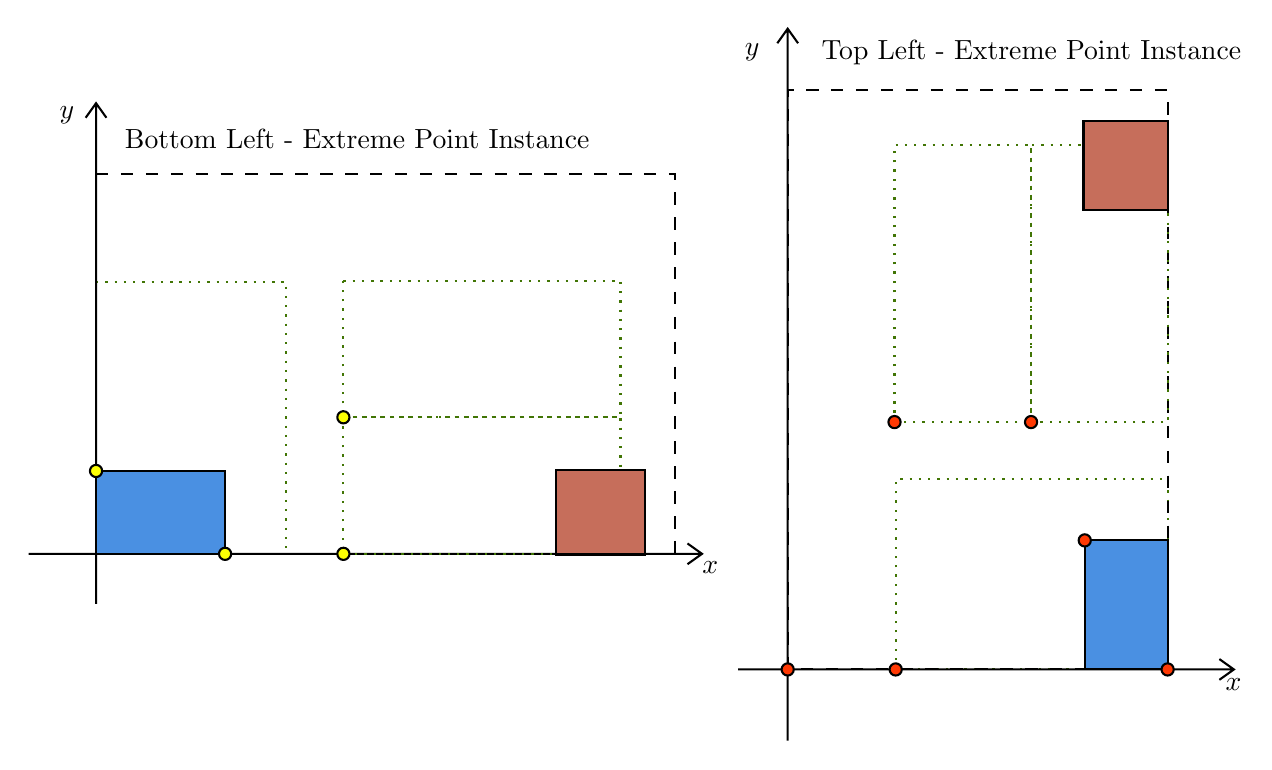
\begin{tikzpicture}[x=0.75pt,y=0.75pt,yscale=-1,xscale=1]
%uncomment if require: \path (0,380); %set diagram left start at 0, and has height of 380

%Shape: Rectangle [id:dp676391404304541] 
\draw  [color={rgb, 255:red, 65; green, 117; blue, 5 }  ,draw opacity=1 ][dash pattern={on 0.84pt off 2.51pt}] (65.44,151.69) -- (157,151.69) -- (157,282.71) -- (65.44,282.71) -- cycle ;
%Shape: Rectangle [id:dp26001178837889305] 
\draw  [color={rgb, 255:red, 65; green, 117; blue, 5 }  ,draw opacity=1 ][dash pattern={on 0.84pt off 2.51pt}] (450.7,338.41) -- (450.7,246.85) -- (581.72,246.85) -- (581.72,338.41) -- cycle ;
%Shape: Rectangle [id:dp532870934725963] 
\draw  [dash pattern={on 4.5pt off 4.5pt}] (65.44,99.66) -- (344.58,99.66) -- (344.58,282.71) -- (65.44,282.71) -- cycle ;
%Shape: Axis 2D [id:dp545947560183275] 
\draw  (33,282.71) -- (357.39,282.71)(65.44,65.6) -- (65.44,306.84) (350.39,277.71) -- (357.39,282.71) -- (350.39,287.71) (60.44,72.6) -- (65.44,65.6) -- (70.44,72.6)  ;
%Shape: Rectangle [id:dp13640021794487145] 
\draw  [fill={rgb, 255:red, 74; green, 144; blue, 226 }  ,fill opacity=1 ] (65.44,242.78) -- (127.61,242.78) -- (127.61,282.71) -- (65.44,282.71) -- cycle ;
%Shape: Ellipse [id:dp4997787088203596] 
\draw  [fill={rgb, 255:red, 252; green, 255; blue, 4 }  ,fill opacity=1 ] (62.5,242.78) .. controls (62.5,241.16) and (63.82,239.84) .. (65.44,239.84) .. controls (67.06,239.84) and (68.38,241.16) .. (68.38,242.78) .. controls (68.38,244.4) and (67.06,245.72) .. (65.44,245.72) .. controls (63.82,245.72) and (62.5,244.4) .. (62.5,242.78) -- cycle ;
%Shape: Ellipse [id:dp9368091558454169] 
\draw  [fill={rgb, 255:red, 252; green, 255; blue, 4 }  ,fill opacity=1 ] (124.67,282.71) .. controls (124.67,281.09) and (125.99,279.77) .. (127.61,279.77) .. controls (129.24,279.77) and (130.55,281.09) .. (130.55,282.71) .. controls (130.55,284.34) and (129.24,285.65) .. (127.61,285.65) .. controls (125.99,285.65) and (124.67,284.34) .. (124.67,282.71) -- cycle ;
%Shape: Rectangle [id:dp10130767347226488] 
\draw  [color={rgb, 255:red, 65; green, 117; blue, 5 }  ,draw opacity=1 ][dash pattern={on 0.84pt off 2.51pt}] (184.62,216.92) -- (318.13,216.92) -- (318.13,282.71) -- (184.62,282.71) -- cycle ;
%Shape: Rectangle [id:dp8859988076373574] 
\draw  [color={rgb, 255:red, 65; green, 117; blue, 5 }  ,draw opacity=1 ][dash pattern={on 0.84pt off 2.51pt}] (184.62,151.14) -- (318.13,151.14) -- (318.13,216.92) -- (184.62,216.92) -- cycle ;
%Shape: Rectangle [id:dp5346376956315015] 
\draw  [fill={rgb, 255:red, 198; green, 110; blue, 91 }  ,fill opacity=1 ] (286.87,242.19) -- (329.77,242.19) -- (329.77,283.04) -- (286.87,283.04) -- cycle ;
%Shape: Ellipse [id:dp5380867242688693] 
\draw  [fill={rgb, 255:red, 252; green, 255; blue, 4 }  ,fill opacity=1 ] (181.68,282.71) .. controls (181.68,281.09) and (182.99,279.77) .. (184.62,279.77) .. controls (186.24,279.77) and (187.55,281.09) .. (187.55,282.71) .. controls (187.55,284.34) and (186.24,285.65) .. (184.62,285.65) .. controls (182.99,285.65) and (181.68,284.34) .. (181.68,282.71) -- cycle ;
%Shape: Circle [id:dp32824759445274065] 
\draw  [fill={rgb, 255:red, 252; green, 255; blue, 4 }  ,fill opacity=1 ] (181.68,216.92) .. controls (181.68,215.3) and (182.99,213.99) .. (184.62,213.99) .. controls (186.24,213.99) and (187.55,215.3) .. (187.55,216.92) .. controls (187.55,218.55) and (186.24,219.86) .. (184.62,219.86) .. controls (182.99,219.86) and (181.68,218.55) .. (181.68,216.92) -- cycle ;
%Shape: Rectangle [id:dp013806976369067359] 
\draw  [dash pattern={on 4.5pt off 4.5pt}] (398.67,338.41) -- (398.67,59.27) -- (581.72,59.27) -- (581.72,338.41) -- cycle ;
%Shape: Axis 2D [id:dp26544149420697416] 
\draw  (374.78,338.41) -- (613.65,338.41)(398.67,29.71) -- (398.67,372.71) (606.65,333.41) -- (613.65,338.41) -- (606.65,343.41) (393.67,36.71) -- (398.67,29.71) -- (403.67,36.71)  ;
%Shape: Rectangle [id:dp4452985784509189] 
\draw  [fill={rgb, 255:red, 74; green, 144; blue, 226 }  ,fill opacity=1 ] (541.79,338.41) -- (541.79,276.23) -- (581.72,276.23) -- (581.72,338.41) -- cycle ;
%Shape: Rectangle [id:dp24524128214266327] 
\draw  [color={rgb, 255:red, 65; green, 117; blue, 5 }  ,draw opacity=1 ][dash pattern={on 0.84pt off 2.51pt}] (515.93,219.23) -- (515.93,85.71) -- (581.72,85.71) -- (581.72,219.23) -- cycle ;
%Shape: Rectangle [id:dp5234703657507643] 
\draw  [color={rgb, 255:red, 65; green, 117; blue, 5 }  ,draw opacity=1 ][dash pattern={on 0.84pt off 2.51pt}] (450.14,219.23) -- (450.14,85.71) -- (515.93,85.71) -- (515.93,219.23) -- cycle ;
%Shape: Rectangle [id:dp9419058705222738] 
\draw  [fill={rgb, 255:red, 198; green, 110; blue, 91 }  ,fill opacity=1 ] (541.2,116.98) -- (541.2,74.08) -- (582.04,74.08) -- (582.04,116.98) -- cycle ;
%Shape: Ellipse [id:dp3331578572136539] 
\draw  [fill={rgb, 255:red, 255; green, 57; blue, 4 }  ,fill opacity=1 ] (450.14,222.17) .. controls (448.52,222.17) and (447.21,220.85) .. (447.21,219.23) .. controls (447.21,217.61) and (448.52,216.29) .. (450.14,216.29) .. controls (451.77,216.29) and (453.08,217.61) .. (453.08,219.23) .. controls (453.08,220.85) and (451.77,222.17) .. (450.14,222.17) -- cycle ;
%Shape: Ellipse [id:dp23570925769851603] 
\draw  [fill={rgb, 255:red, 255; green, 57; blue, 4 }  ,fill opacity=1 ] (515.93,222.17) .. controls (514.31,222.17) and (512.99,220.85) .. (512.99,219.23) .. controls (512.99,217.61) and (514.31,216.29) .. (515.93,216.29) .. controls (517.56,216.29) and (518.87,217.61) .. (518.87,219.23) .. controls (518.87,220.85) and (517.56,222.17) .. (515.93,222.17) -- cycle ;
%Shape: Ellipse [id:dp6429169005498813] 
\draw  [fill={rgb, 255:red, 255; green, 57; blue, 4 }  ,fill opacity=1 ] (398.67,341.35) .. controls (397.04,341.35) and (395.73,340.03) .. (395.73,338.41) .. controls (395.73,336.78) and (397.04,335.47) .. (398.67,335.47) .. controls (400.29,335.47) and (401.6,336.78) .. (401.6,338.41) .. controls (401.6,340.03) and (400.29,341.35) .. (398.67,341.35) -- cycle ;
%Shape: Ellipse [id:dp5636473664839672] 
\draw  [fill={rgb, 255:red, 255; green, 57; blue, 4 }  ,fill opacity=1 ] (450.7,341.35) .. controls (449.08,341.35) and (447.76,340.03) .. (447.76,338.41) .. controls (447.76,336.78) and (449.08,335.47) .. (450.7,335.47) .. controls (452.33,335.47) and (453.64,336.78) .. (453.64,338.41) .. controls (453.64,340.03) and (452.33,341.35) .. (450.7,341.35) -- cycle ;
%Shape: Ellipse [id:dp310194773919646] 
\draw  [fill={rgb, 255:red, 255; green, 57; blue, 4 }  ,fill opacity=1 ] (581.72,341.35) .. controls (580.1,341.35) and (578.78,340.03) .. (578.78,338.41) .. controls (578.78,336.78) and (580.1,335.47) .. (581.72,335.47) .. controls (583.34,335.47) and (584.66,336.78) .. (584.66,338.41) .. controls (584.66,340.03) and (583.34,341.35) .. (581.72,341.35) -- cycle ;
%Shape: Ellipse [id:dp4413085834987862] 
\draw  [fill={rgb, 255:red, 255; green, 57; blue, 4 }  ,fill opacity=1 ] (541.79,279.17) .. controls (540.17,279.17) and (538.85,277.86) .. (538.85,276.23) .. controls (538.85,274.61) and (540.17,273.29) .. (541.79,273.29) .. controls (543.41,273.29) and (544.73,274.61) .. (544.73,276.23) .. controls (544.73,277.86) and (543.41,279.17) .. (541.79,279.17) -- cycle ;

% Text Node
\draw (46.39,65.64) node [anchor=north west][inner sep=0.75pt]    {$y$};
% Text Node
\draw (356.09,284.84) node [anchor=north west][inner sep=0.75pt]    {$x$};
% Text Node
\draw (77.86,76.79) node [anchor=north west][inner sep=0.75pt]   [align=left] {Bottom Left - Extreme Point Instance};
% Text Node
\draw (376.52,35.3) node [anchor=north west][inner sep=0.75pt]    {$y$};
% Text Node
\draw (608.21,341.49) node [anchor=north west][inner sep=0.75pt]    {$x$};
% Text Node
\draw (413.49,33.94) node [anchor=north west][inner sep=0.75pt]   [align=left] {Top Left - Extreme Point Instance};


\end{tikzpicture}

    %}
    \caption{Extreme Point instances for some coordinate changes of \cref{fig:support_planes}}
    \label{fig:ep_coordinate_changes}
\end{figure}

Given \cref{eq:ep_can_pack} to check if a considered placement would lead to a feasible insertion, a set of items to pack $I$, a set $s$ and a bin $b \in B^s$, the heuristic that will output the new best possible feasible insertion for the given set of items is outlined in Algo. \ref{algo:sp_bestinsertion}.

\begin{algorithm}[hp]
    \DontPrintSemicolon
    \SetAlgoLined
    \SetKwInOut{Input}{input}
    \SetKwInOut{Output}{output}
    \Input{$Z, I, T$}
    \Output{$p$}
    \ForAll{$(z, I_{support}, I_{upper}) \in Z$}{
        $P \gets \emptyset$\;
        \ForAll{possible coordinate changes}{
            $p \leftarrow (z, \emptyset)$\;
            $T^\prime \gets \text{empty AABB tree}$\;
            \CommentSty{//Initialize reference points}\;
            $refPoints \gets (0,0)$\;
            \ForAll{$i \in I_{support}$}{
                $refPoints \gets refPoints \cup \{(x_i, y_i)\}$\;
            }
            \ForAll{$i \in I_{upper}$}{
                $refPoints \gets refPoints \cup \{(x_i + w_i, y_i), (x_i, y_i + d_i)\}$\;
            }
            $sort(refPoints)$ \CommentSty{// Based on euclidean distance from $(0,0)$}\;

            \CommentSty{//Create a feasible insertion for the given items}\;
            \ForAll{$i \in I$}{
                \CommentSty{//Evaluate first possible placement}\;
                \ForAll{$(x,y) \in refPoints$}{
                    $(x_i, y_i, z_i) \gets (x, y, z)$\;
                    \If{$EPCanPlace(i, T, T^\prime)$}{
                        $EPInsertRect(p, i, T^\prime, refPoints)$ \CommentSty{// alg. \ref{algo:ep_insert_rect}}\;
                        break\;
                    }
                    $(w_i, d_i) \gets (d_i, w_i)$ \CommentSty{//Try rotating $i$}\;
                    \If{$EPCanPlace(i, T, T^\prime)$}{
                        $EPInsertRect(p, i, T^\prime, refPoints)$ \CommentSty{// alg. \ref{algo:ep_insert_rect}}\;
                        break\;
                    }
                    $(w_i, d_i) \gets (d_i, w_i)$ \CommentSty{//Restore original $i$ rotation}\;
                }
            }
            \If{$p \neq (z, \emptyset)$}{
                $P \gets P \cup \{ p \}$\;
            }
        }
        $sort(P)$ \CommentSty{//Sorted as in \cref{ssec:scoring_insertions}}\;
        \If{$P \neq \emptyset$}{
            \Return{first element of $P$}
        }
    }
    \Return{none}
    \caption{SP Best Insertion \label{algo:sp_bestinsertion}}
\end{algorithm}
\begin{algorithm}[htb] 
    \DontPrintSemicolon
    \SetAlgoLined
    \SetKwInOut{Input}{input}
    \SetKwInOut{Output}{output}
    \Input{ $p, i, T, refPoints$}
    $refPoints \gets refPoints \setminus \{ (x_i, y_i) \}$\;
    $refPoints \gets refPoints \cup \{(x_i + w_i, y_i), (x_i, y_i + d_i)\}$\;
    $sort(refPoints)$ \CommentSty{// Based on euclidean distance from $(0,0)$}\;
    $p.I \gets p.I \cup \{ i \}$\;
    $AABBInsert(i, T^\prime)$ \CommentSty{//\cref{sec:problem_state:aabbtree}}\;
    \Return
    \caption{EP Insert Rect \label{algo:ep_insert_rect}}
\end{algorithm}

\paragraph*{Commit Extension}
We now describe an extension to $Commit$ (Algo. \ref{algo:state_commit}) that updates the structures needed by SP.

When a plane is filled, new insertions become less likely to be feasible.
To avoid evaluating planes where no insertion is possible we develop a mechanism to prune dead planes.

Since best insertions for a bin are always evaluated by considering lower planes first, if all the insertions in $Expand$ (Algo. \ref{algo:state_successor}) happened over a $z_{min}$, then we can safely remove the opened planes with $z < z_{min}$ for that bin.
Let us introduce a $z^s_{min}$ variable that is updated during the $Expand$ phase with the minimum $z$ of all the insertions on bin $b$.
Once the best states are computed and $Commit$ is called, we can use $z^s_{min}$ to prune planes in each $b \in B^s$.
Other operations are also necessary in the $Commit$ algorithm to allow SP to update its data structures accordingly to the insertion.

Let $s$ be a state and let $p$ be an insertion where each packed item $i \in I_p$ in bin $b_p$ has $z^s_i$ within tolerance of $z$.
The algorithm which updates the structures for a given bin $b$ is represented by algorithm \ref{algo:sp_commit}.
This new algorithm can be used as the last step of the $Commit$ algorithm for each $b \in B^{s^\prime}$.

\begin{algorithm}[H] \label{algo:sp_commit}
    \DontPrintSemicolon
    \SetAlgoLined
    \SetKwInOut{Input}{input}
    \SetKwInOut{Output}{output}
    \SetSideCommentRight
    \Input{$s_b, I, z, z_{min}, t$}
    \Output{$s^\prime_b$}
    \CommentSty{//Filter bad planes}\;
    $P^\prime \leftarrow planes \setminus \{ \forall S_z \in planes : z \le z_{min} \}$\;
    \CommentSty{//Apply insertion}\;
    $B \leftarrow placed \cup I$\;
    $U \leftarrow unpacked \setminus I$\;
    $T \leftarrow aabb$\;
    \ForAll{$i \in I$}{
        $T \leftarrow InsertAABB(i, T)$ \CommentSty{//If balanced $O(log(n))$}\; %TODO: specify balanced
        $generate \leftarrow true$\;
        % O(|P'|)
        \ForAll{$S^\prime_z \in P^\prime$}{ %TODO: specify balanced
            \CommentSty{//Based on the distance from the top of the item}\;
            $dz \leftarrow S^\prime_z.z - i.z_{max}$\;
            \If{$0 \le dz \le t$}{
                $generate \leftarrow false$\;
                $S^\prime_z.I_{support} \leftarrow S^\prime_z.I_{support} \cup i$\;
            } \ElseIf{$dz < 0$}{
                $S^\prime_z.I_{upper} \leftarrow S^\prime_z.I_{upper} \cup i$\;
            }
        }

        \If{$generate$}{
            $P^\prime \leftarrow P^\prime \cup (i.z_{max}, \{i\}, \emptyset)$\;
        }
    }
    \Return{$Update(s_b, P^\prime, B, U, T)$}
    \caption{SP Apply and Filter}
\end{algorithm}

\subsection{Sorting Insertions}
\label{ssec:scoring_insertions}%
Similarly to the sorting of states (\cref{ssec:scoring_states}), an ordering function is also needed to evaluate different insertions for the same set of items.
Given the lexicographic ordering formulation in \cref{def:lexicographic_ordering}, a few new functions can be calculated and stored inside an insertion to help in the evaluation.
Given $T$ as the AABB Tree that represents the bin where the insertion is going to happen, and given one of the inserted items $i \in I_p$, we define functions that use the tree to calculate useful metrics:
\begin{itemize}
    \item $CloseItems(i, T)$: which returns the number of packed items that are close to $i$,
    \item $CloseSameHeight(i, T)$: which returns the number of packed items in the tree that are close to $i$ and with its same height,
    \item $CloseSameShape(i, T)$: which returns the number of packed items in the tree that are close to $i$ and with its same shape,
    \item $TotalSupportedArea(i, T)$: which returns the total base area of $i$ which is supported by other items.
\end{itemize}
We can then sort insertions $p$, given $T$ as the AABB tree of the bin where the insertion will happen, with a lexicographic ordering as follows:
\begin{itemize}
    \item $f_1(p) = -\sum\limits_{i \in I_p}{CloseSameShape(i, T)} - |I_p|$: maximize number of items inserted (of the same shape) that are close to already packed items of the same shape,
    \item $f_2(p) = -\sum\limits_{i \in I_p}{(w^s_i d^s_i + w^s_i d^s_i h^s_i)}$: maximize the sum of the area and volume of each packed item,
    \item $f_3(p) = \max\limits_{i \in I_p}(z^s_i + h_i)$: minimize the maximum height of the inserted items,
    \item $f_4(p) = \sum\limits_{i \in I_p}{TotalSupportedArea(i, T)}$: minimize the support area available to the inserted items,
    \item $f_5(p) = -\sum\limits_{i \in I_p}{CloseSameHeight(i, T)} - |I_p|$: maximize the number of items inserted (of the same height) that are close to already packed items of the same height,
    \item $f_5(p) = -\sum\limits_{i \in I_p}{CloseItems(i, T)} - |I_p|$: maximize the number of items inserted that are close to already packed items.
\end{itemize}
It is noted that preferring feasible insertions that minimize the supported area of each item as in $f_4$ is inspired by other works on spacing from the literature.
As shown in \cite{elhedhli2019three}, overly satisfying the support constraint can lead to unbalanced bins.
Minimizing the supported area of each item leads to minimizing the perimeter of overlap between items which in turn results in more balanced bins that have better spacing between items.